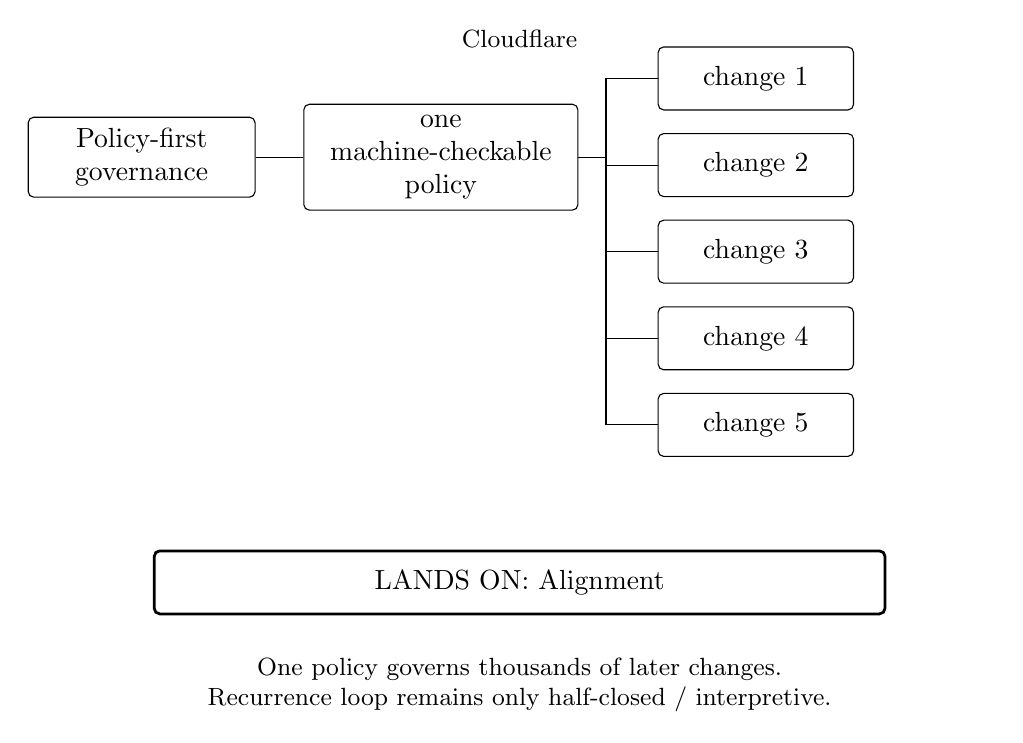
\begin{tikzpicture}[x=1cm,y=1cm,font=\magefigurefont\fontsize{10}{12}\selectfont,
box/.style={draw=black,fill=white,rounded corners=2pt,align=center,text width=3cm,minimum height=8mm,inner sep=4pt},
gate/.style={box,line width=1pt},note/.style={align=center,fill=white,inner sep=1pt,font=\magefigurefont\fontsize{9}{11}\selectfont},
edge/.style={-{Stealth[length=2mm]},line width=.6pt},optional/.style={edge,dashed},
every node/.style={text=black,execute at begin node={\hyphenpenalty=10000\exhyphenpenalty=10000}}]
\node[note,text width=12cm] (t5) at (0,1.5) {Cloudflare};
\node[box,text width=2.6cm] (entry) at (-4.8,0) {Policy-first governance};
\node[box,text width=3.2cm] (hub) at (-1,0) {one machine-checkable policy};
\draw[draw] (entry) -- (hub);
\node[box,text width=2.2cm] (p0) at (3,1.0) {change 1};
\draw (hub.east) -- ++(.35,0) |- (p0.west);
\node[box,text width=2.2cm] (p1) at (3,-0.10000000000000009) {change 2};
\draw (hub.east) -- ++(.35,0) |- (p1.west);
\node[box,text width=2.2cm] (p2) at (3,-1.2000000000000002) {change 3};
\draw (hub.east) -- ++(.35,0) |- (p2.west);
\node[box,text width=2.2cm] (p3) at (3,-2.3000000000000003) {change 4};
\draw (hub.east) -- ++(.35,0) |- (p3.west);
\node[box,text width=2.2cm] (p4) at (3,-3.4000000000000004) {change 5};
\draw (hub.east) -- ++(.35,0) |- (p4.west);
\node[gate,text width=9cm] (land) at (0,-5.4) {LANDS ON: Alignment};
\node[note,text width=12cm] (t20) at (0,-6.7) {One policy governs thousands of later changes.\\ Recurrence loop remains only half-closed / interpretive.};
\end{tikzpicture}
